\section{Programming Protocol-Independent Packet Processor} \label{sec:p4}

P4 is a programming language allows us to config a special design switch. In P4, we can tell the switch how to parse a packet by identifying the packet header. Furthermore, we can store or edit the content inside packet header and forward it to the right port or even drop it. 

\begin{figure}[tbh]
    \centering
    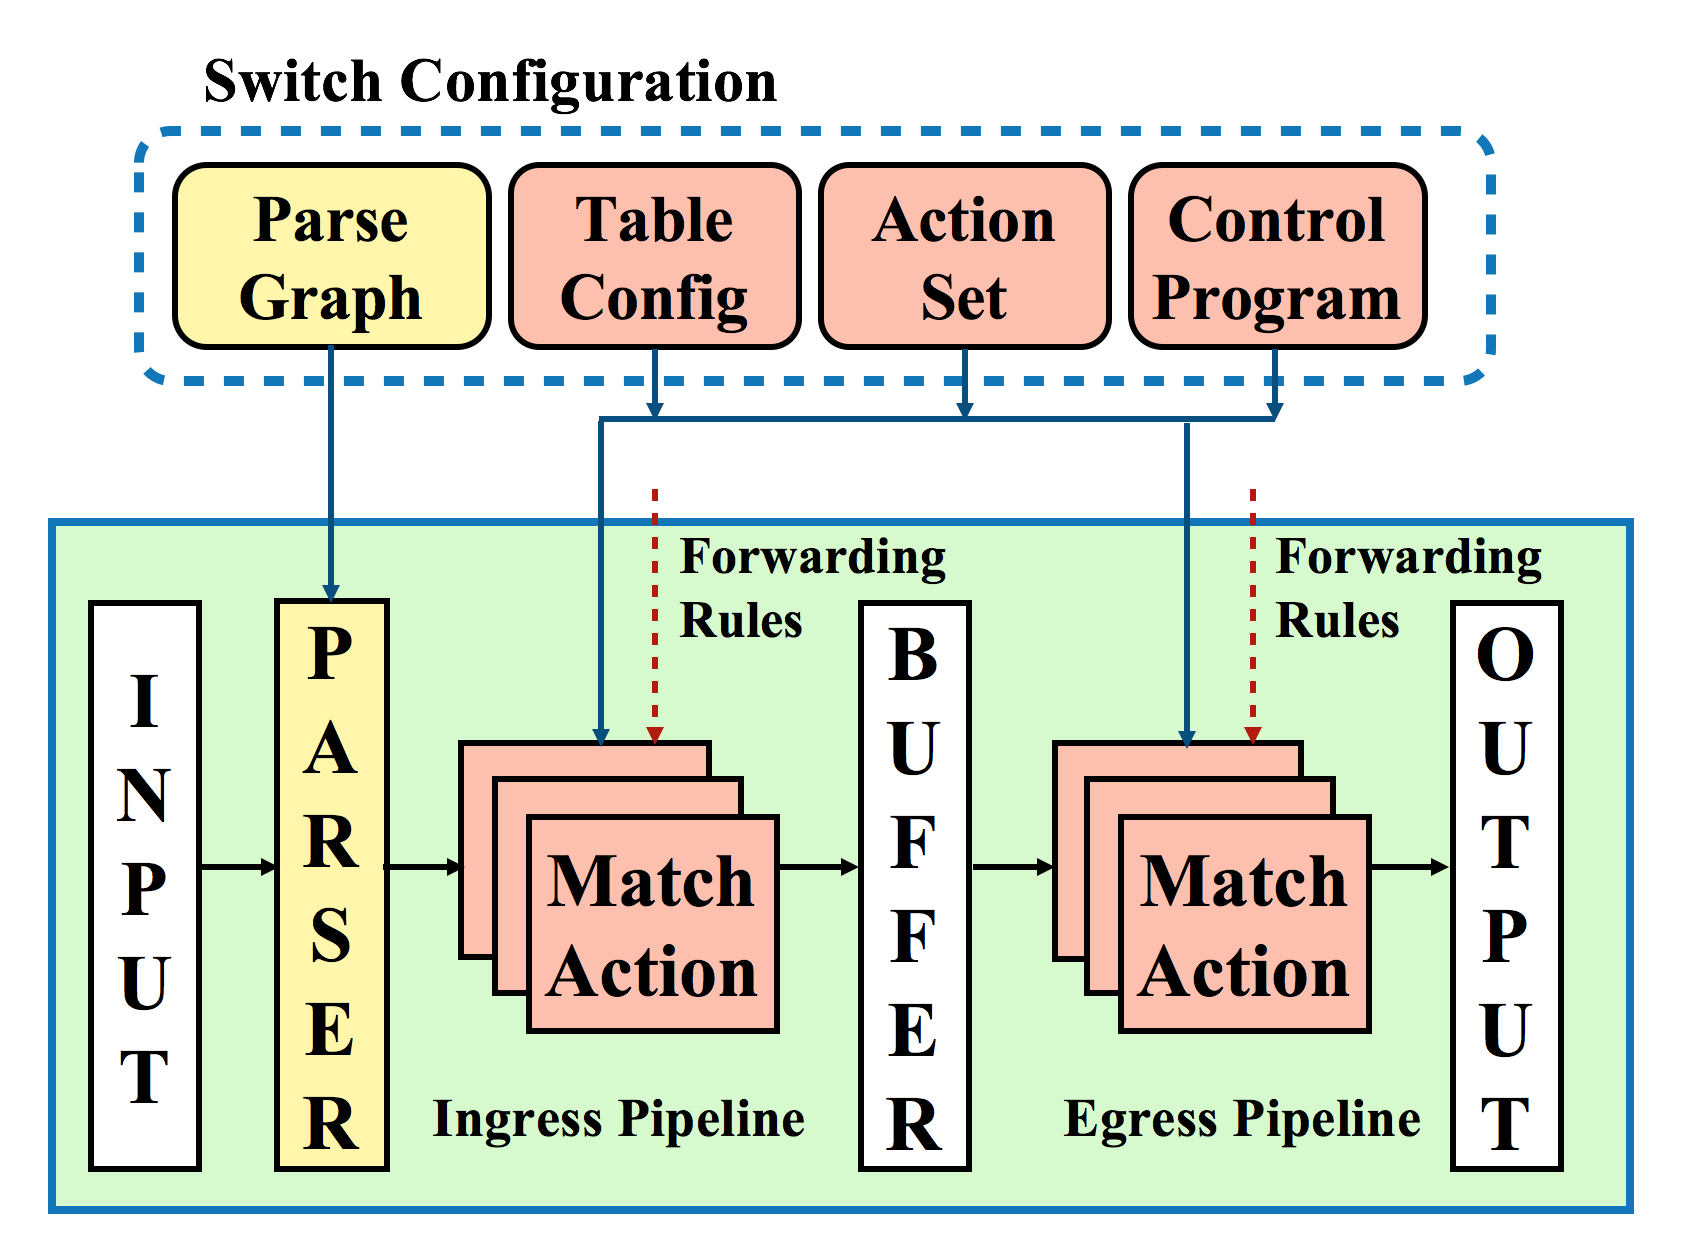
\includegraphics[width=.50\textwidth]{fig/p4.png}
    \caption{P4 Abstract~\cite{BDGI+14}}
    \label{p4}
\end{figure}

Fig.~\ref{p4} is a standard P4 switch diagram drawn by P4 Organization. Companies like Barefoot has designed some ASICs to run P4 program. It has many pipelines for us to deploy our P4 program in match and action table. P4 program actually consists of 4 parts, parse graph, table config, action set, control program. Parse graph tells P4 switch how to parse a packet. It could parse kinds of packets if we write it correctly. The other three parts works together. We have to implement many tables to match the field of packet header and actions. Each match+action table has a set of actions, we can match the packet to do the correction. The control program is more like a script exist both in ingress pipeline and egress pipeline. This control program will decide the order of math+action table. If the packet passes the two control pipeline, it will be pushed into output buffer and then send out by interface.